\documentclass[9pt]{extarticle}

\usepackage{tgpagella}
\usepackage[scaled]{helvet}
\usepackage[T1]{fontenc}
\usepackage{fontspec}
\usepackage[a4paper,left=2cm,right=2cm,top=2cm,bottom=2.5cm]{geometry}
\usepackage{titlesec}
\usepackage{authblk}
\usepackage{multicol}
\usepackage{enumitem}
\usepackage{graphicx}
\usepackage[labelsep=period,center]{caption}
\usepackage{subcaption}
\usepackage{float}
\usepackage[numbers]{natbib}
\usepackage{url}
\usepackage[hidelinks]{hyperref}
\usepackage{xcolor}
\usepackage[numbib]{tocbibind}
\usepackage{amsmath}
\usepackage{tabularx}
\usepackage{booktabs}

\defaultfontfeatures{LetterSpace=0}

\graphicspath{ {./images/} }

% centered column for tables with tabularx
\newcolumntype{Y}{>{\centering\arraybackslash}X}

% bibliography section formatting
\bibliographystyle{vancouver}
\makeatletter
\renewcommand\@biblabel[1]{#1.} %from [1] to 1
\makeatother
\renewcommand\UrlFont{\color{blue}\rmfamily}

% captions for figures and tables
\captionsetup[figure]{labelfont={sf,bf},textfont={up,md,sf}}
\captionsetup[table]{labelfont={sf,bf},textfont={up,md,sf}}

% fonts
% this syntax assumes that the font files are in the same directory as the .tex file
\setsansfont[Path=./,
UprightFont = *, 
BoldFont = *_Bold,
ItalicFont = *_Italic,
BoldItalicFont = *_Bold_Italic
]{Arial}

\setromanfont[Path=./,
UprightFont = *, 
BoldFont = *_Bold,
ItalicFont = *_Italic,
BoldItalicFont = *_Bold_Italic
]{Times_New_Roman}

\setmainfont[Path=./,
UprightFont = *, 
BoldFont = *_Bold,
ItalicFont = *_Italic,
BoldItalicFont = *_Bold_Italic
]{Times_New_Roman}

\setmonofont{DejaVuSansMono}

% formatting of section and subsection titles
\titleformat{\section}[hang]{\bfseries\sffamily\fontsize{10pt}{10pt}\selectfont}{\thesection.$\quad$}{0pt}{}
  
\titleformat{\subsection}[runin]{\bfseries\sffamily\itshape\fontsize{9pt}{10pt}\selectfont}{}{0pt}{}[:$\;$] % i've tried a lot of things... and THIS is what i came up with :(

\titlespacing*{\section}{0pt}{8pt plus 4pt minus 2pt}{0pt plus 2pt minus 2pt}
\titlespacing*{\subsection}{0pt}{4pt plus 2pt minus 2pt}{0pt plus 2pt minus 2pt}

% formatting of lists
%\setlist[itemize]{leftmargin=*,itemsep=0mm}
\setlist[itemize]{itemsep=0mm}
\setlist[description]{leftmargin=*,itemsep=0mm}
\setlist[enumerate]{leftmargin=*,itemsep=0mm}

% title, authors, affiliation
\renewcommand*{\Authfont}{\fontsize{12pt}{14pt}\bfseries\itshape\sffamily}
\renewcommand*{\Affilfont}{\fontsize{10pt}{12pt}\bfseries\sffamily\upshape}

\title{
    \vspace{-2em}
    \centering
    \fontsize{14pt}{14pt}
    \bfseries
    \sffamily
    Title Must be in 14 pt. Helvetica or Arial Bold: Required by Eurodisplay 2020 Digest Formatting
    \vspace{-0.3em}
}

\author[*]{Andrew M. Peli-Smith}
\author[**]{Hiroyuki Furukawa\vspace{-0.6em}}
\affil[*]{Schepens Eye Research Institute, Boston MA}
\affil[**]{Sharp Corporation, Osaka, Japan\vspace{-1em}}

\date{} % has to be empty, so it won't show up

\begin{document}

\maketitle

\pagestyle{empty}
\thispagestyle{empty} % needed to remove nasty page number created by \maketitle

\renewcommand{\baselinestretch}{1} % single spacing

\setlength{\parindent}{0cm} % no indentation

\setlength\columnsep{1.25cm} % distance between columns (no idea if correct)

\begin{multicols}{2} % two column layout

\section*{Abstract}

{
\bfseries\itshape
This sample file was produced for Palisades Convention Management and modified by the Eurodisplay 2020 organizers for use by authors of Eurodisplay 2020 Conference Publication Papers \& Posters.
Authors are encouraged and requested to use this template to produce their final submission for the electronic and print publications.
Kindly follow this sample file so that the publication will have the same or very similar formatting throughout and provide attendees with a good source of venue documentation.
}

\section*{Author Keywords}

Use semi-colons; between; your choice; of keywords.
Including keywords is strongly encouraged because this section enhances the search functions of most electronic publications.

\section{Introduction and Formatting Guidelines Part 1}

This format is to be used for submissions that are published in the conference publications.
We wish to give this volume a consistent, high-quality appearance.
We therefore ask that authors follow some simple guidelines.
In essence, you should format your paper exactly like this document.
The easiest way is simply to download a template from the conference website and replace the content with your own material. 

\subsection{Page Size \& Margins}

Be sure that your paper is 21 × 29.7 cm (A4 size) with .2cm margin at the top, left and right sides and 2.5cm margin at the bottom.
A4 is a standard page size option in most applications and programs.
\textbf{\textit{Letters sized submissions will be returned to the authors to fix.}}

\subsection{Title of Paper}

The title of your paper should be in 14 pt. Helvetica or Arial Bold (see above). 
Capitalize the \underline{F}irst \underline{L}etter of \underline{M}ain \underline{W}ords in the \underline{T}itle (\underline{M}ost \underline{N}ouns), except a, an, the, conjunctions (and, but, or, for, …), and prepositions (of, to, in, on, …).

\subsection{No Headers or Footers}

Your final submission \textbf{MUST NOT} contain any footer or header string information at the top or bottom of each page nor any page numbering.
The submissions will be paginated in a determined order by the chairs and page numbers added to the PDF later.

\subsection{Author's Full Names}

Authors’ names should appear in 12 pt. Helvetica or Arial Bold Italic.
Multiple authors with the same affiliation can be grouped together; use a 2 or 3 column setup for authors of different affiliations.
Authors must include their \textbf{full first names}.
This is very helpful for proper indexing of authors with multiple submissions.
Please make sure that each author’s name is listed as first, middle, and last name.

\section{Continued Formatting Guidelines}

\subsection{Affiliation Information}

Please include your department, main affiliation, complete location and contact author’s email address.
All this information should appear in 10 pt. Helvetica or Arial Bold (not italic, see above).

\subsection{Section Heads}

Section heads should appear in 10 pt. Helvetica or Arial bold with 6 to 12 points of additional space above.
Section heads should remain with at least 2 lines of body text immediately following them when they appear at the bottom of a column or page.

\subsection{Sub-Section Heads}

Sub-section heads should appear in 10 pt. Arial Italic and as paragraph lead-ins, with 6 pts of additional space above or before.
See this paragraph as an example.

\subsection{Body Text}

The body text of your submission should be 9 pt. Times or Times New Roman, single spaced with an additional 4 to 6 points of space after each paragraph. Do not indent paragraphs and be sure the body text is justified (except for bulleted or numbered lists).

\subsection{Bulleted and Numbered Lists}

All bulleted and numbered lists should not have any additional indent and the text should indent hang.
See the samples within this template.

\subsection{Table and Figure Captions}

Figure captions should appear centered under the corresponding figure and be set in 9 pt. Helvetica or Arial Bold.
Table captions should appear centered above the corresponding table and be set in 9 pt. Helvetica or Arial Bold.
These items should appear as close to where they are cited as possible.
See Section 5 for more information.

\subsection{Wide Tables and Figures}

Wide tables and figures should be placed at the top or bottom of the page where they are mentioned — not within the middle of a page with text above and below.

\subsection{References}

Should be numbered and be 9 pt. Times or Times New Roman, single spaced with an additional 4 to 6 points of space after each reference.
The section should be made ragged right to prevent url breaks.


\section{PDF Creation}

We recommend that you produce a PDF version of your submission well before the final deadline.
Your PDF file must be compliant with the requirements at:

\url{http://www.scomminc.com/pp/pcm/DW-distilling-settings.htm}

Test your PDF file by viewing and/or printing it.

\subsection{Two Examples on How to Include Equation}

See how the math strings were added in Equations \ref{eqn:sum} and \ref{eqn:matrix}: % TODO ref

\begin{equation}
    \label{eqn:sum}
    d = \epsilon + \sum_{i = 1}^{8} m_i w_i
\end{equation}

\begin{equation}
    \label{eqn:matrix}
    \begin{bmatrix} Y \\ U \\ V \end{bmatrix}
    =
    \begin{bmatrix}
        0.2126 & 0.7152 & 0.0722 \\
        -0.1146 & -0.3854 & 0.5000 \\
        0.5000 & -0.4542 & -0.0458
    \end{bmatrix}
    \begin{bmatrix} R \\ G \\ B \end{bmatrix}
\end{equation}

\begin{figure}[H]
    \centering
    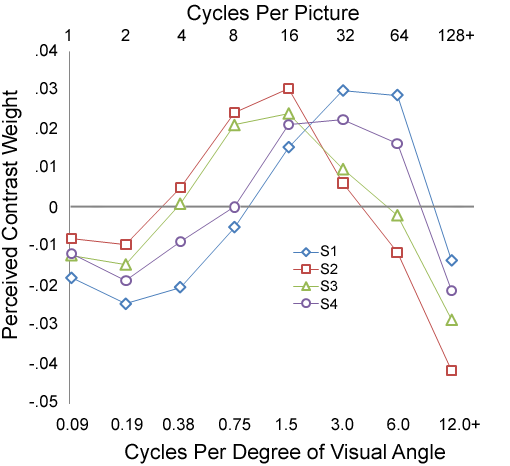
\includegraphics[width=\linewidth]{cycles}
    \caption{Note the position of the figure caption UNDER the image.}
    \label{fig:cycles}
\end{figure}

{\renewcommand{\arraystretch}{1.2}
\begin{table}[H]
\centering
\caption{Sample of a Table Caption Above the Table. Tag number should appear in 9 pt. Helvetica or Arial Bold and body not bold.}
    \begin{tabularx}{\linewidth}{ |c|Y|Y|c| } 
    \hline
        \multicolumn{2}{|c|}{\textbf{LC Parameters}} & \multicolumn{2}{c|}{\textbf{cell parameters}} \\
    \hline
    $K_{11}$ & 11.6 pN & \textit{d} & 2 µm \\
    \hline
    $K_{33}$ & 20.8 pN & (bottom, top) & (0, 0) \\
    \hline
    $P_{o}$ & 0.388 µm & \multicolumn{2}{c|}{number of grids} \\
    \hline
    $e_{||}$ & 17.8 × $\epsilon_o$ & $N_y$ & 50 \\
    \hline
    $K_{11}$ & 11.6 pN & \textit{d} & 2 µm \\
    \hline
\end{tabularx}
\label{table:table_lable}
\end{table}}

As an example, use this setup for a numbered list:

\begin{enumerate}
    \item See below for the examples for a bulleted list
    \item If space is needed, reduce the 6 pts of extra space after each listed item to only 3 pts. 
    \item In addition, be sure that all your “open and close” quotes match up 
\end{enumerate}

\subsection{Filler text paragraph}

A recommendation should be made to every federal or state agency that as part of any reactive chemical incident investigation, the public release of a summary of the incident, root causes, and lessons learned.

As an example, use this setup for a bulleted list:

\begin{itemize}
    \item Screening evaluation
    \item Computation evaluation 
\end{itemize}


\section{Language, Style, and Content}

Spelling and punctuation may use any dialect of English (e.g., British, Canadian, US, etc.) provided this is done consistently.
Hyphenation is optional.
To ensure suitability for an international audience, please pay attention to the following:

\begin{itemize}
    \item Write in a straightforward style. Use simple sentence structures. Try to avoid long sentences and complex sentence structures. Use semicolons carefully.
    \item Use common and basic vocabulary (e.g., use the word “unusual” rather than the word “arcane”).
    \item Briefly define or explain all technical terms. The terminology common to your practice/discipline may be different in other design practices/disciplines.
    \item Spell out all acronyms the first time they are used in your text. For example, OLED (organic light-emitting diode).
    \item Explain local references (e.g., not everyone knows all city names in a particular country).
    \item Explain “insider” comments. Ensure that your whole audience understands any reference whose meaning you do not describe.
    \item Explain colloquial language and puns. Understanding phrases like “red herring” requires a cultural knowledge of English. Humor and irony are difficult to translate.
    \item Use unambiguous forms for culturally localized concepts, such as times, dates, currencies and numbers (e.g., “1-5-97” or “5/1/97” may mean 5 January or 1 May, and “seven o'clock” may mean 7:00 am or 19:00).
    \item Be careful with the use of gender-specific pronouns (he, she) and other gender-specific words (chairman, manpower, man-months). Use inclusive language (e.g., she or he, they, chair, staff, staff-hours, person-years) that is gender-neutral. If necessary, you may be able to use “he” and “she” in alternating sentences, so that the two genders occur equally often. 
\end{itemize}

\section{Recommendations for Your Figures \& Images}

These are recommendations to ensure good print reproduction of the images, figures, and illustrations utilized in your submission.

\subsection{(a) Colors and Black \& White (Gray Scale) Print Testing}

If you have any images in color, please print your paper out in black and white to ensure that the tones and screens used in your images or figures reproduce well in black and white, too.
However, your images will appear in full color in any distributed electronic proceedings and in the digital library. 

\subsection{(b) Resolution \& CMYK}
Images in your document should be at least 300 or 600 dpi for quality reproduction and saved as .tif images (or other compatible format that supports print quality resolution).
When creating or revising your images for inclusion in the paper, we recommend choosing CMYK (and not RGB) as the color profile. 

\begin{figure}[H]
    \centering
    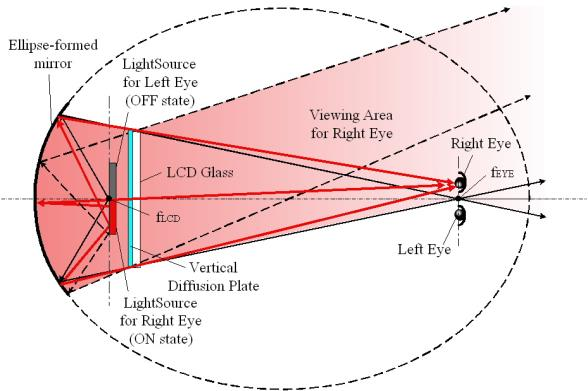
\includegraphics[width=\linewidth]{ellipse}
    \caption{370mmx470mm MOTFT backpanel processed from a Gen-2.5 color filter production line and a 4.8” FC}
    \label{fig:ellipse}
\end{figure}

\end{multicols}

\begin{figure*}[h]
    \centering
    \begin{subfigure}[c]{7.75cm}
        \centering
        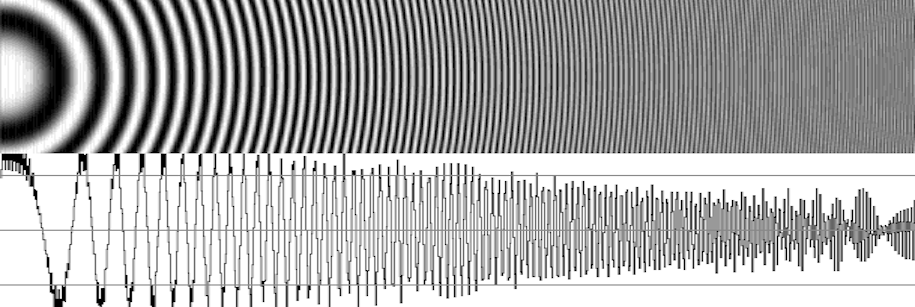
\includegraphics[width=\textwidth]{wave1}
        \caption{RGBYe (sampling interval: 1/2)}
        \label{fig:wave1}
    \end{subfigure}
    \hfill
    \begin{subfigure}[c]{7.75cm}
        \centering
        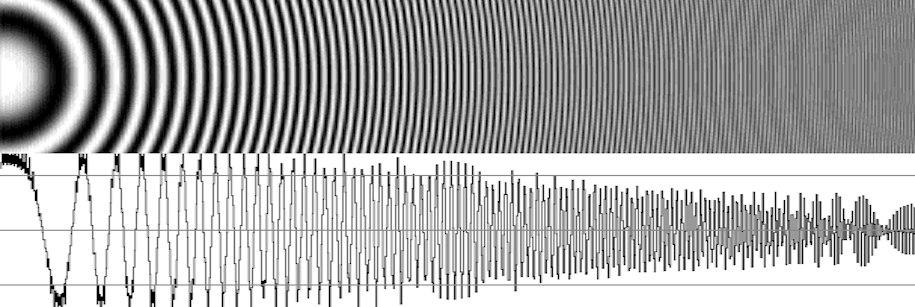
\includegraphics[width=\textwidth]{wave2}
        \caption{RGBCy (sampling interval: 1/2)}
        \label{fig:wave1}
    \end{subfigure}
    \caption{Wide Figure Caption. Should appear in \textbf{9 pt. Helvetica or Arial Bold and Centered Under} Figure. This is also a good example of how to keep figures with multiple parts together using a table setup.}
    \label{fig:waves}
\end{figure*}

\begin{multicols}{2}

\subsection{(c) .TIF (.EPS), .JPEG and .PNG images}
.TIFs are preferred for press applications where quality takes priority over file size.
When .TIFs are compressed (LZW compression option when saving out of Photoshop, for example), no image data is lost, thus ensuring maximum quality.

A .JPEG is a compressed image format designed to keep the file size small, which makes it ideal for use in web graphics.
To do this, the .JPEG format actually deletes image data from the image.
The higher the level of compression, the more data is removed.
This is referred to as a lossy compression system.
On a printout, the removed data tends to show up as blocky areas of a solid color.
If you have to use JPEG files make sure to use a low compression (large file size) and check for visible artifacts.
Generally JPEG is well suited for photos but not for drawings. 

Since a .PNG file doesn’t compress the image like other lossy formats like .JPEG do, quality doesn’t diminish as much when the image is in the .PNG format.
.JPEG files are useful when the image is low contrast, but .PNGs are better when dealing with sharp contrast like when there are lines or text in the image, as well as large areas of solid color.

\subsection{(d) Rules/Lines}
Rules used in your graphs, tables or charts must be at least 0.5+ pt. and black for quality reproduction. 

\subsection{(e) Fonts}
If your figure uses custom or any non-standard font, the characters may appear differently when printed in the proceedings.
Remember to check your figure creation to ensure that all fonts are embedded or included in the figure correctly.
\textbf{\textit{BE SURE THAT YOUR IMAGES DO NOT CONTAIN ANY TYPE 3 FONTS.}}

\subsection{(f) Transparencies}
If a figure or image is assembled from multiple images, the images must be embedded, and layers flattened or grouped together properly in the file, not lined.
Transparencies need to be flattened.

\subsection{(g) Position}
Images and figures are best at the top or bottom of a column for narrow images/figures.
Wide figures must appear at the very top or very bottom of a page (see the sample images included in this sample file).

\section{Discussion and/or Conclusion Section}

Include discussion of your results and your conclusion of the tests.
Balance of this paragraph is filler text — results demonstrate that the perceptual impact of an image, and the way its contrast is interpreted by an observer, is dependent on the structure of the image, thereby suggesting that perceived contrast of complex imagery is not an entirely passive process.
Individual differences in the weighting functions also may correspond with previously described differences in preference for video enhancement by normal observers.  

\section{Impact of your Research}

Include discussion of your results and your conclusion of the tests.
Balance of this paragraph is filler text — results demonstrate that the perceptual impact of an image, and the way its contrast is interpreted by an observer, also may correspond with previously described differences in preference for video enhancement by normal observers.  

\section{Acknowledgements}

Authors, please be sure to include any acknowledgements of funding or grants received, as may be required by the benefactor to have your research published.
Author A.C. Browns wants to acknowledge the funding received from NSF (grant no. 123456) or Supported in part by NIH grants EY0X957, EY1G093.

\section{References}

\textbf{Note:} As of the 2020 technical program and digest, authors should use the Vancouver reference style. 

Last name of author followed by initial, et al. for more than six authors, etc. Example below \cite{davis_using_2007}:

\begingroup
\renewcommand{\section}[2]{} % do not print section title
\raggedright
\bibliography{literature}
\endgroup

\end{multicols}

\end{document}
